\chapter{Wyniki}
\label{cha:wyniki}

\section{Gry 3-osobowe}
\label{sec:N3nzal}

\paragraph{Równania standardowe}
\label{sec:r_stan}
\begin{wrapfigure}{rh}{0.5\textwidth}
    \centering
    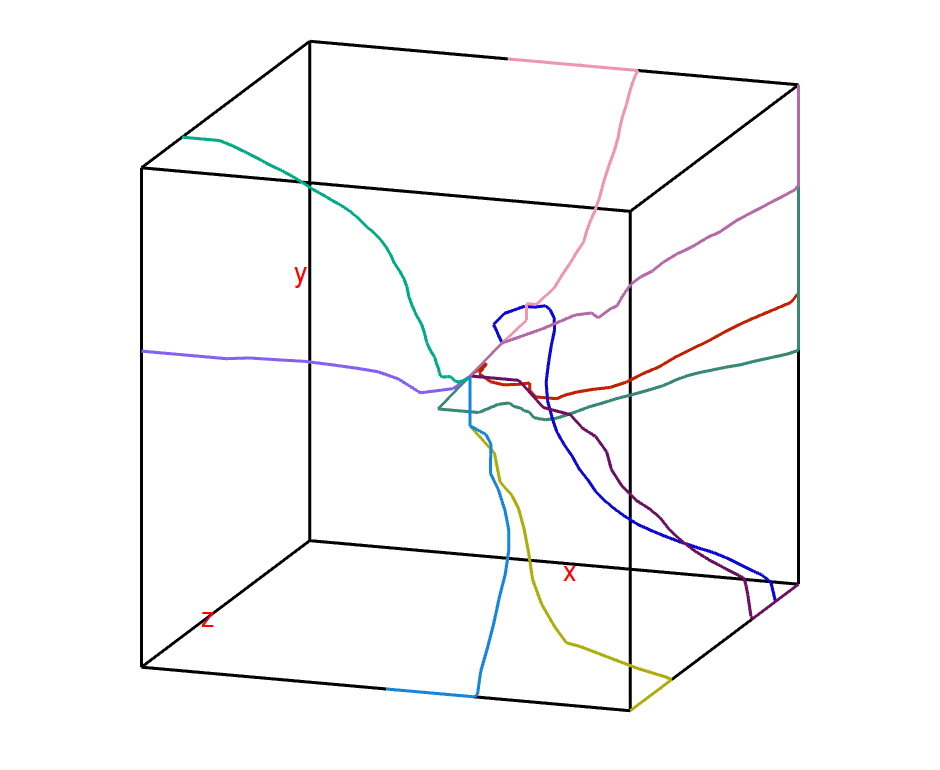
\includegraphics[width=0.5\textwidth]{pict/wyniki/stand100_10.png}   
    \caption{Równania standardowe: 100 partii, 10 instancji}
	\label{fig:stand100_10} 
\end{wrapfigure}

Analiza teoretyczna równań wskazała $(\frac{1}{2},\frac{1}{2},\frac{1}{2})$ jako punkt stabilny. Wynikało to z założenia gry o pełnej informacji, co nie jest spełnione dla symulacji, której funkcje opuszczają centrum sześcianu. Osiągnięcie przez funkcję krawędzi sześcianu oznacza zawiązanie koalicji, po czym funkcja przesuwa się po krawędzi dążąc do wierzchołka. Analizując tabelkę \ref{tab:krawedz_prawd} można ją także odnieść do równań standardowych by dojść do wniosku że funkcja powinna osiągać punkt stabilności na krawędzi i nie poruszać się dalej. Byłoby tak gdyby błąd szacowania prawdopodobieństw przeciwników był odpowiednio mały. Szacowanie prawdopodobieństw dane jest przez $\frac{nast_{j}}{liczba_{partii}}$. Wynika z tego, że wystarczy kilka zagrań przeciwników niezgodnych z zawartą koalicją, aby gracz szacujący ich prawdopodobieństwa nie mógł stwierdzić, że ich realne prawdopodobieństwa wynoszą 0 lub 1. Co pokazuje rysunek \ref{fig:stand100_10}, na którym widać funkcje o wielu punktach przegięcia. Szybkość dążenia do wierzchołków będzie malała wraz z czasem spędzonym na krawędzi, gdyż 
\[\lim_{nast_j\rightarrow liczba_{partii} \wedge liczba_{partii} \rightarrow \infty} \frac{nast_j}{liczba_{partii}} \in \{0,1\} \]

%---------------------------------------------------------------------------------------------------------------------------------------------------------
\paragraph{Równania replikatorów}
\label{sec:r_repl}

\begin{figure}
	\centering
	\begin{tabular}{c|c}
		\centering
		\subfloat[100 partii \label{fig:repl100_10}]{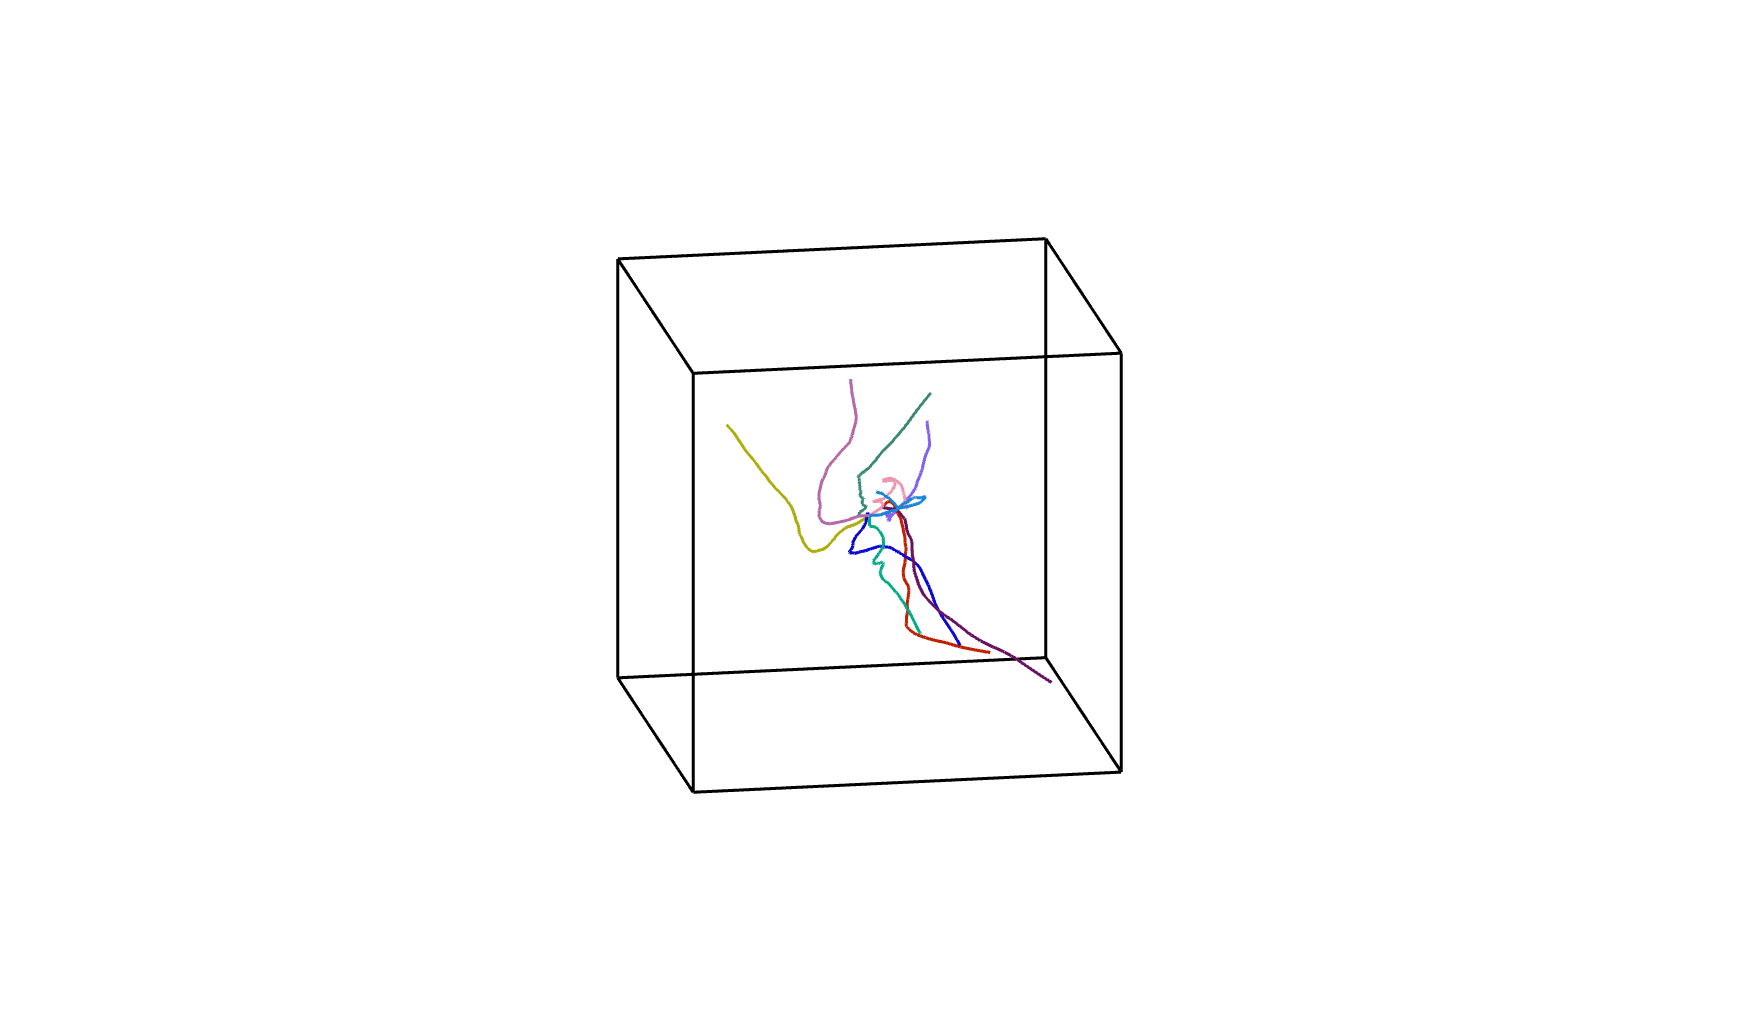
\includegraphics[width=.45\textwidth]{pict/wyniki/repl100_10.png}} 
		&
		\subfloat[250 partii \label{fig:repl250_10}]{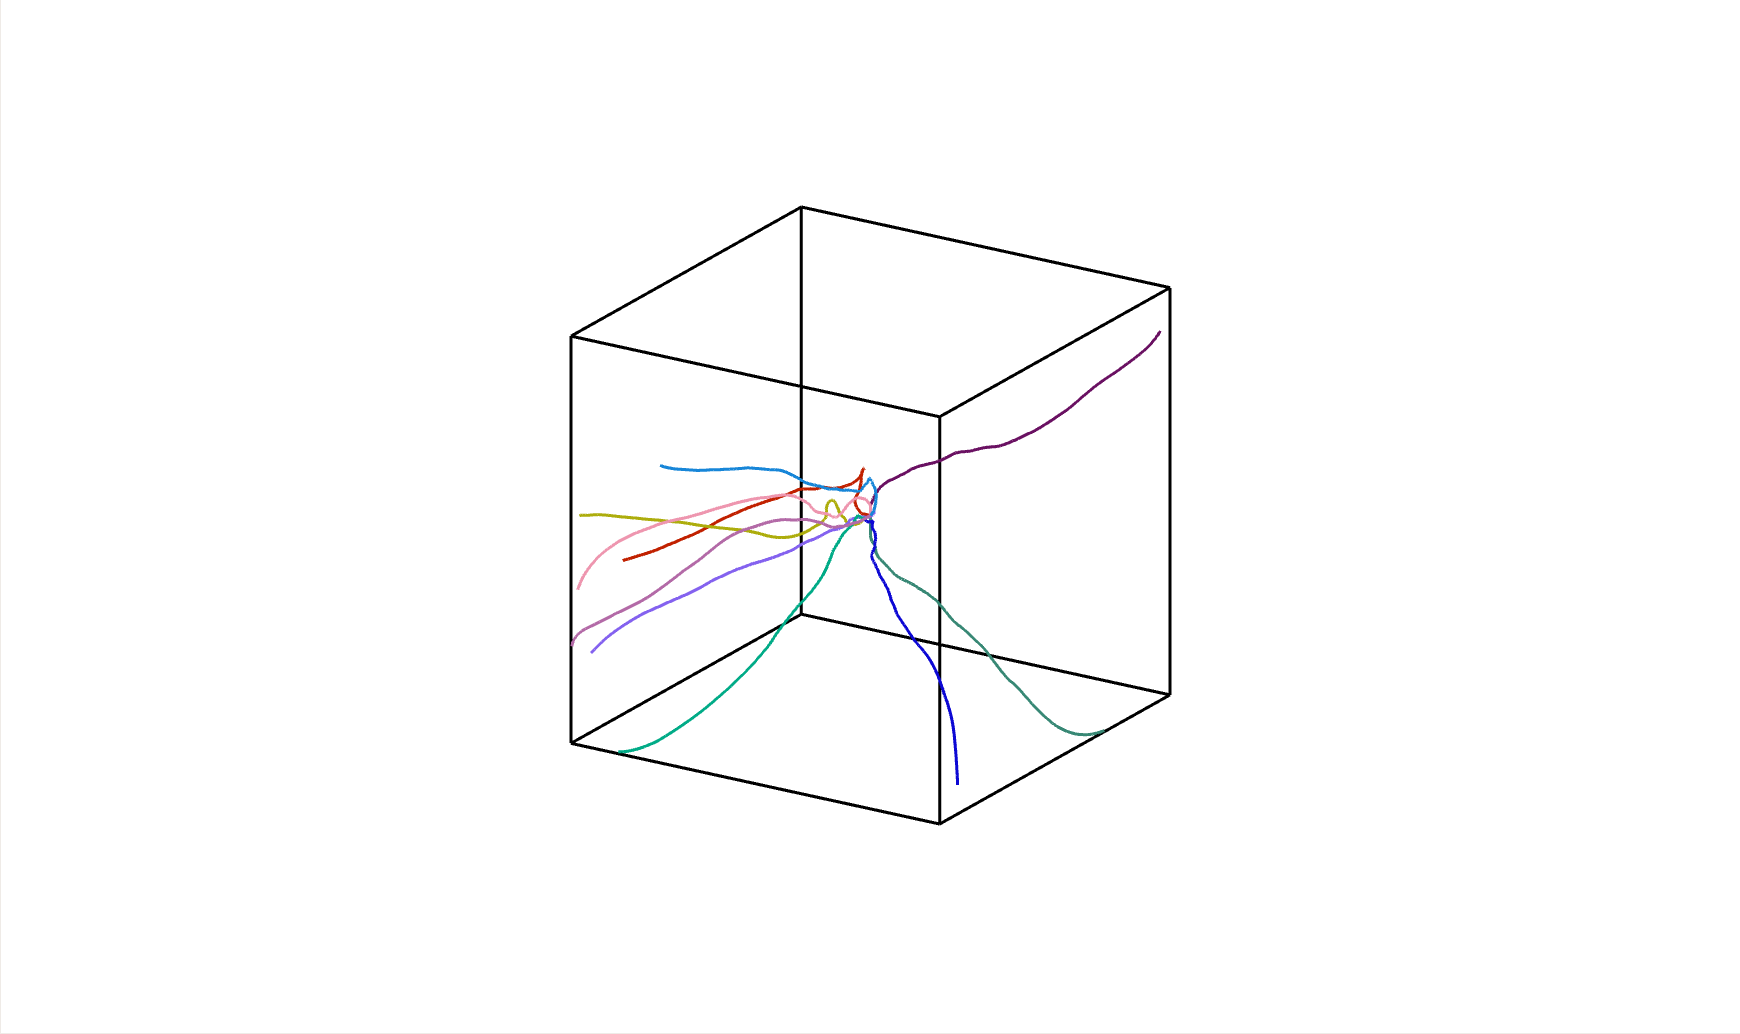
\includegraphics[width=.45\textwidth]{pict/wyniki/repl250_10.png}}
		\\ \hline
		\subfloat[1000 partii \label{fig:repl1000_10}]{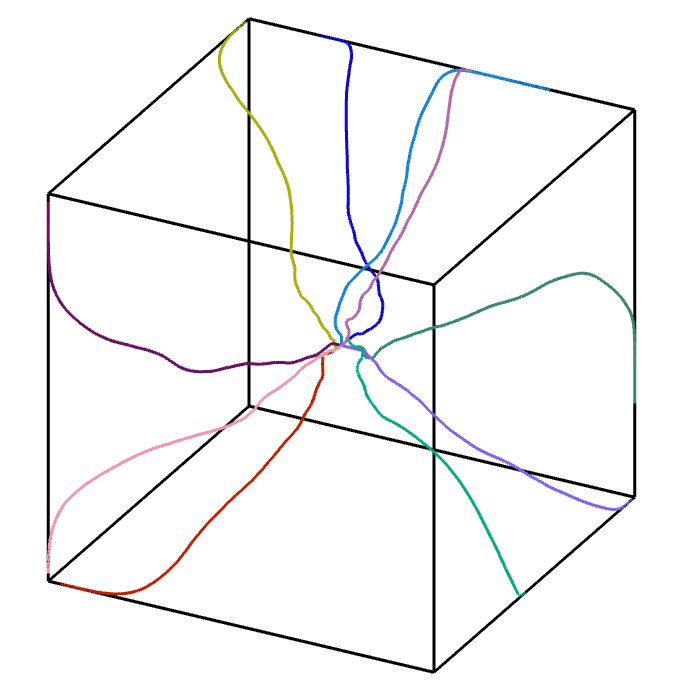
\includegraphics[width=.45\textwidth]{pict/wyniki/repl1000_10.png}}
		&
		\subfloat[10000 partii \label{fig:repl10000_10}]{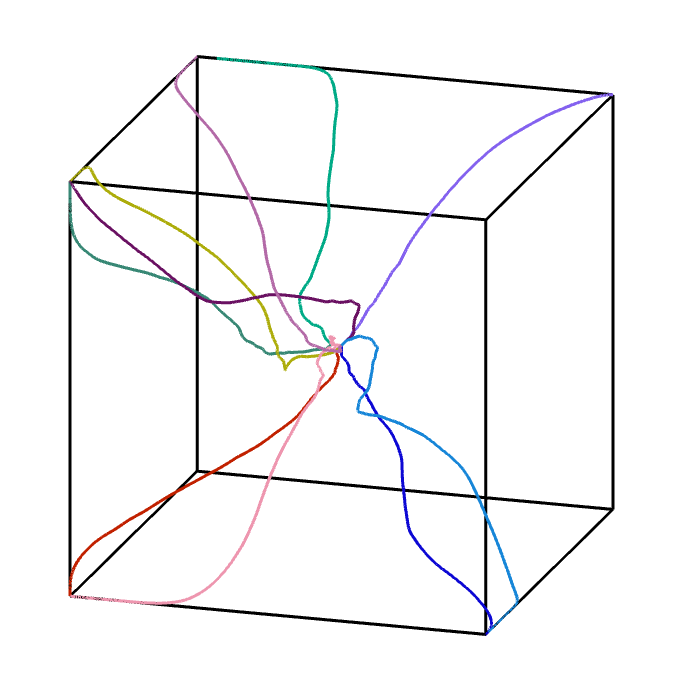
\includegraphics[width=.45\textwidth]{pict/wyniki/repl10000_10.png}}
	\end{tabular}
\caption{Równania replikatorów: 10 instancji}
\label{fig:repl_10}
\end{figure}
Równań replikatorów charakteryzują się mniejszej dynamiką gry w stosunku do równań standardowych. Przyczyną jest człon $x(1-x)$, którego maksimum wynosi $0.25$. Daje to czterokrotnie mniejsze $\Delta p$ w punkcie $(\frac{1}{2}, \frac{1}{2}, \frac{1}{2})$. Na krańcach dziedziny $<0,1>$ wspomniany człon szybko dąży do 0 (przypomina wielomian węzłowy Lagrange'a), co znacznie opóźnia osiągnięcie koalicji. Widać to porównując rysunki \ref{fig:stand100_10} oraz \ref{fig:repl100_10}. Dopiero rysunki \ref{fig:stand100_10} oraz \ref{fig:repl10000_10}, gdzie gra używająca równań replikatorów wykonała ich 100 razy więcej niż gra używająca równań standardowych pokazują liczbę partii potrzebną do osiągnięcia podobnych miejsc w przestrzeni sześcianu.
\begin{wrapfigure}{rh}{0.5\textwidth}
    \centering
    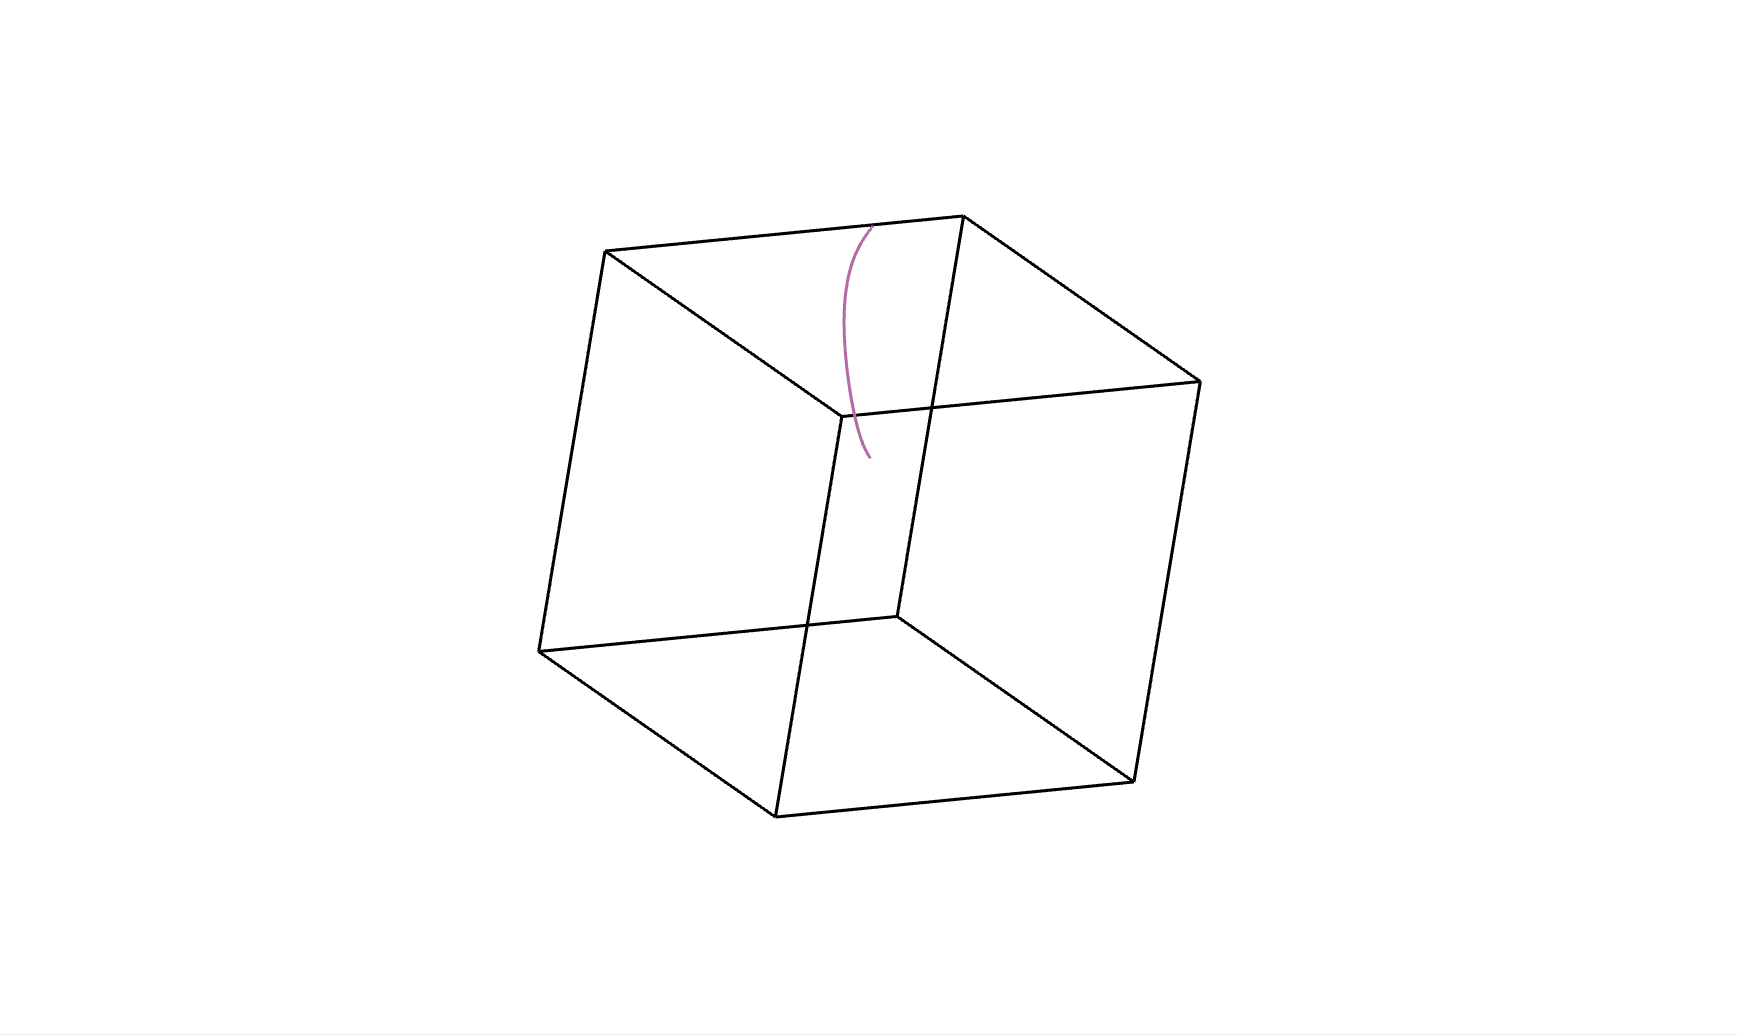
\includegraphics[width=0.5\textwidth]{pict/wyniki/repl_realp_mp_300_10.png}   
    \caption{Równania replikatorów, gra o pełnej informacji: 300 partii, 10 instancji}
	\label{fig:realp} 
\end{wrapfigure}
Analiza stabilności pokazała, że każda krawędź sześcianu powinna być punktem stabilnym, potwierdza to rysunek \ref{fig:realp}. Natomiast symulacja \ref{fig:repl1000_10} pokazuje przemieszczanie się funkcji ku wierzchołkom. Znów powodem jest błąd w szacowaniu prawdopodobieństwa przeciwników. Nie występuje on jednak we wszystkich instancjach gry, na przykład w jasno-zielonej rozgrywce \ref{fig:repl1000_10} widać, że funkcja nieznacznie porusza się po krawędzi, co świadczy o mniejszym błędzie szacowania prawdopodobieństwa w stosunku do innych rozgrywek. Analiza stabilności wskazuje, że punkty $(0,0,0)$ oraz $(1,1,1)$ nie są stabilne, czego dowodem jest iż żądna z symulacji do nich nie zmierza. Co więcej pierwszy i ostatni wiersz tabelki \ref{tab:krawedz_prawd} nie może wystąpić w symulacji. Osiągnięcie punktu $(0,0,\xi )$ lub $(1,1,\xi )$, gdzie $\xi$ nie jest w pobliżu $0$ lub $1$, nie jest możliwe w symulacji. Oznaczałoby to zawiązanie sojuszu pomiędzy graczami, których zagrania nie mają na celu zawiązania między nimi koalicji. Potwierdzają to symulacje z których żadna nie dochodzi do krawędzi wychodzących z punktów $(0,0,0)$ oraz $(1,1,1)$.

%---------------------------------------------------------------------------------------------------------------------------------------------------------
\section{Gry N-osobowe}
\label{sec:N3zal}
\begin{figure}
	\centering
	\begin{tabular}{c|c}
		\centering
		\subfloat[500 partii, 19 graczy \label{fig:Nrepl_g500p19}]{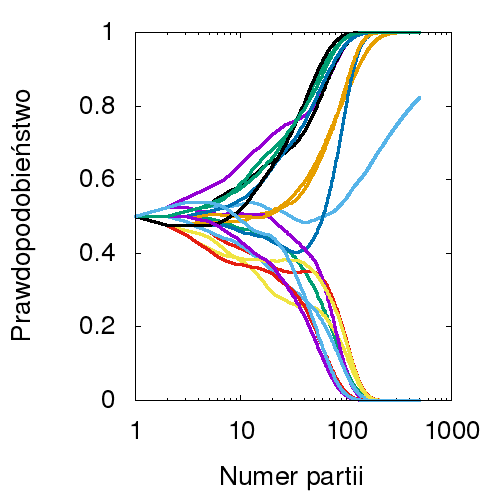
\includegraphics[width=.45\textwidth]{pict/wyniki/g500p19.png}} 
		&
		\subfloat[500 partii, 20 graczy \label{fig:Nrepl_g500p20}]{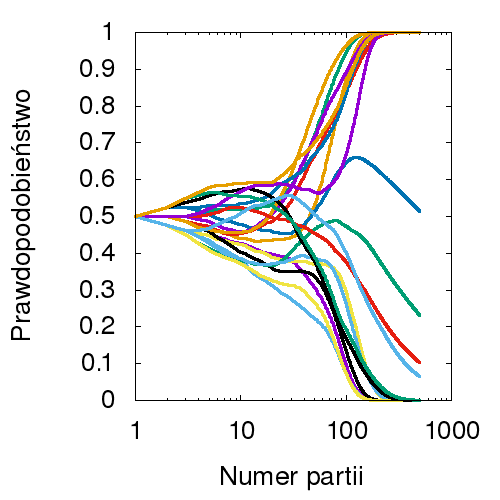
\includegraphics[width=.45\textwidth]{pict/wyniki/g500p20.png}}
		\\ \hline
		\subfloat[500 partii, 21 graczy \label{fig:Nrepl_g500p21}]{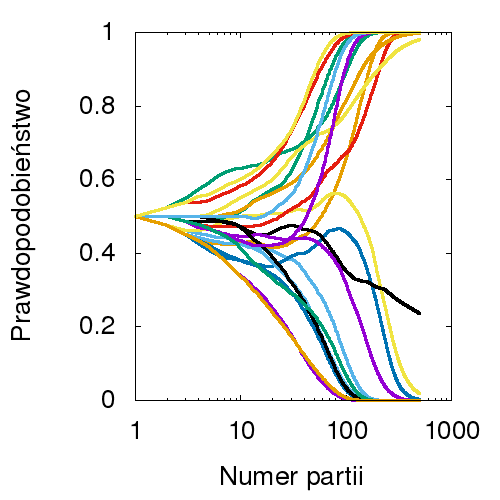
\includegraphics[width=.45\textwidth]{pict/wyniki/g500p21.png}}
		&
		\subfloat[10000 partii, 200 graczy \label{fig:Nrepl_g10000p200}]{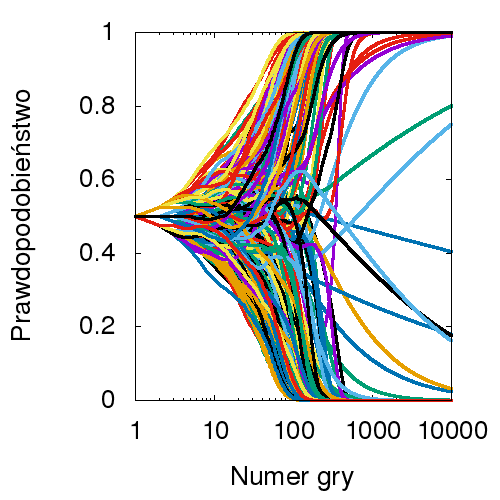
\includegraphics[width=.45\textwidth]{pict/wyniki/g10000p200.png}}
	\end{tabular}
\caption{Gry N-osobowe}
\label{fig:repl_10}
\end{figure}
W grze gdzie ustawionych w okręgu jest $N$ graczy, spodziewamy się że istotnym czynnikiem będzie parzystość ich liczby. Teoretyczna liczba graczy mogących nie znaleźć koalicjanta wynosi $< N\text{ mod }2, \left\lfloor \frac{N}{3} \right\rfloor >$. W grze o parzystej liczbie graczy zawsze istnieje rozwiązanie, które gwarantuje każdemu graczowi przynależność do koalicji. Natomiast w grach o nieparzystej liczbie graczy musi istnieć co najmniej jeden zawodnik, który nie zawrze sojuszu (posiadanie prawdopodobieństwa 0 lub 1, nie jest równoznaczne z byciem w sojuszu, co pokazały symulacje dla 3-graczy, kiedy funkcje dążyły do wierzchołków). Maksymalna liczba graczy bez sojuszu może być maksymalnie połową liczby graczy będących w sojuszy( maksymalnie co trzeci gracz może być bez sojuszy z zaokrągleniem w dół ). Gdyby była większa oznaczałoby to że istnieją pary sąsiadujących graczy, którzy nie są w żadnej koalicji. Tak sytuacja nie może mieć miejsca, ponieważ omawiane pary stałyby się koalicjami. 

Przy dużej ilości gier jednocześnie można zaobserwować sytuacje, w których sąsiedzi zawodnika stosują w przewadze jedną taktykę. Co prowadzi do dokładnego szacowania ich prawdopodobieństw. Skutkiem tego jest gracz nie dokonujący zmian w swoim zachowaniu, co wynika z tabelki \ref{tab:krawedz_prawd}. Przypadek taki można zaobserwować na rysunku \ref{fig:Nrepl_g10000p200}, oznaczony kolorem czarnym.

































